\documentclass[11pt,letterpaper]{article}
\usepackage[utf8]{inputenc}

%ola 
%----- Configuración del estilo del documento------%
\usepackage{epsfig,graphicx}
\usepackage[left=2.5cm,right=2.5cm,top=1.8cm,bottom=2.3cm]{geometry}
%------ Paquetes matematicos --------%
\usepackage{amsmath}
\usepackage{amssymb}
\usepackage{amsthm}
\usepackage{amsmath}
\usepackage{tabularx}
\usepackage[numbers]{natbib}
\usepackage{fancyhdr}
\usepackage{lastpage}
\usepackage{verbatim}
\usepackage[shortlabels]{enumitem}
\usepackage{venndiagram}
\usepackage{xcolor}
\usetikzlibrary{shapes.geometric}
\renewcommand{\proofname}{Demostración}
\usepackage{cancel}
\usepackage{hyperref}

%%Para la portada
%\usepackage[top=1in, left=0.9in, right=1.25in, bottom=1in]{geometry}
%\usepackage[utf8]{inputenc}
\usepackage[T1]{fontenc}
\usepackage[utf8]{inputenc}
\usepackage[spanish,es-nodecimaldot,es-tabla]{babel}
\usepackage{graphicx}
\usepackage{tocloft}
\graphicspath{{./figs/}}
\usepackage{setspace}

% Paquete para codigo 
\usepackage{minted}

%Color bibi
\definecolor{bibi}{RGB}{0,103,148}
% Otros colores

\begin{document}
	
    \begin{titlepage}
	\thispagestyle{empty}
	\begin{minipage}[c][0.17\textheight][c]{0.25\textwidth}
		\begin{center}
			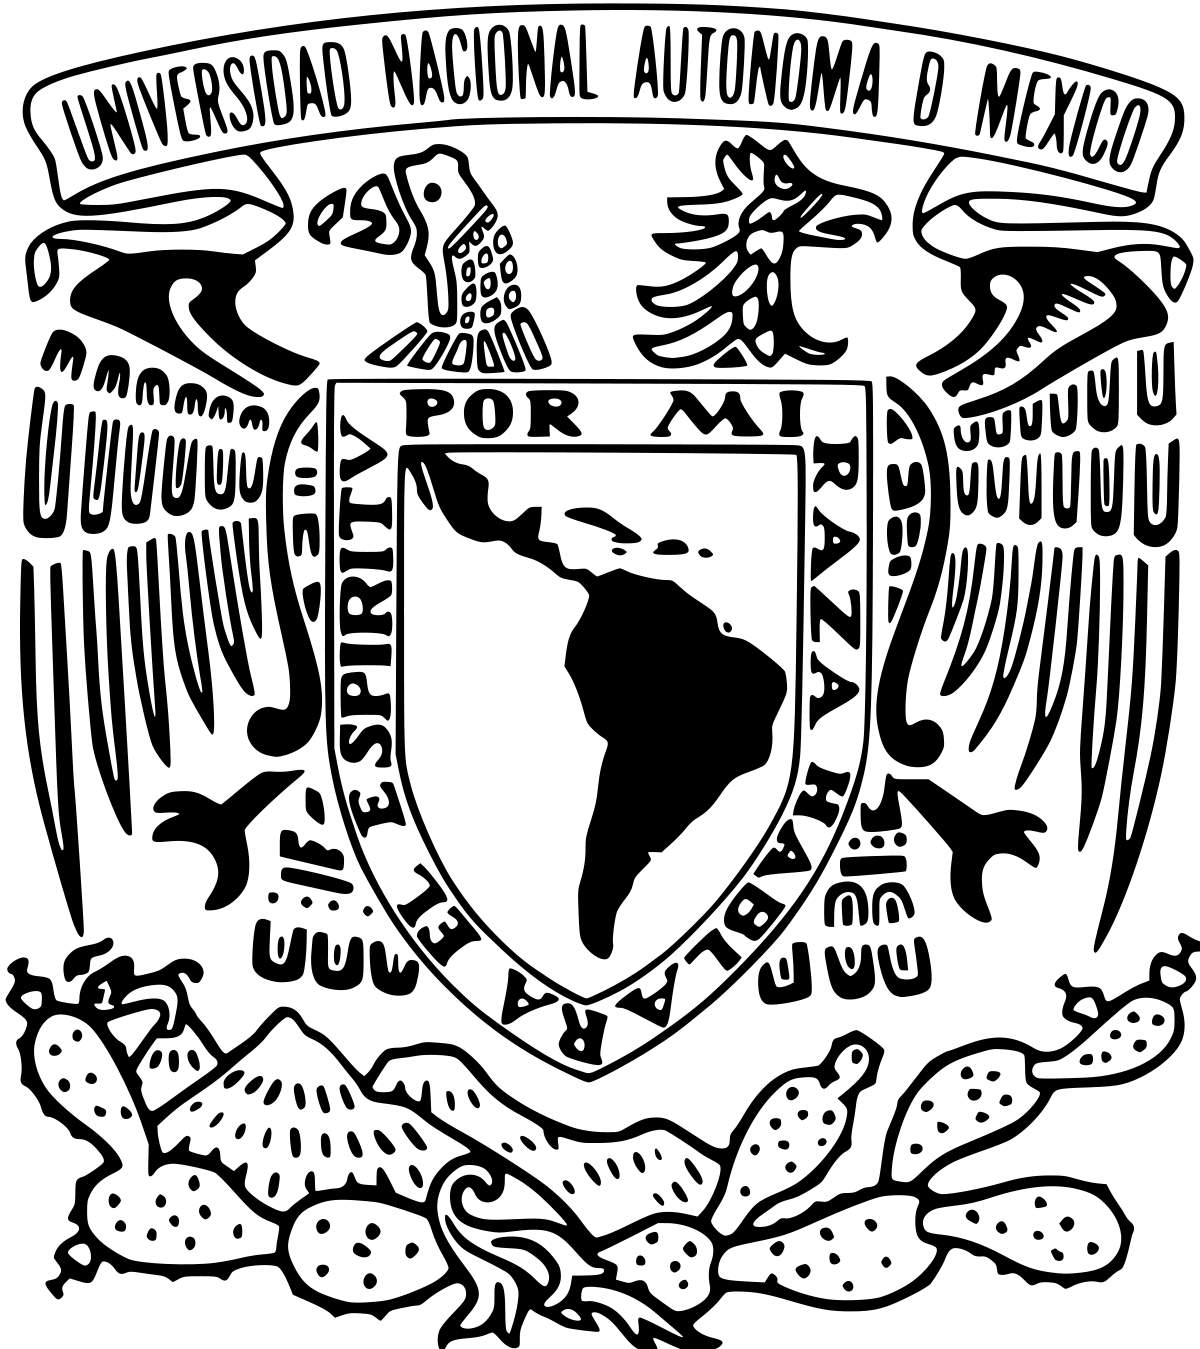
\includegraphics[width=3.5cm, height=3.5cm]{resources/Logo_UNAM.png}
		\end{center}
	\end{minipage}
	\begin{minipage}[c][0.195\textheight][t]{0.75\textwidth}
		\begin{center}
			\vspace{0.3cm}
			\textsc{\large Universidad Nacional Aut\'onoma de M\'exico}\\[0.5cm]
			\vspace{0.3cm}
			\hrule height2.5pt
			\vspace{.2cm}
			\hrule height1pt
			\vspace{.8cm}
			\textsc{Facultad de Ciencias}\\[0.5cm] %
		\end{center}
	\end{minipage}
	
	\begin{minipage}[c][0.81\textheight][t]{0.25\textwidth}
		\vspace*{5mm}
		\begin{center}
			\hskip2.0mm
			\vrule width1pt height13cm 
			\vspace{5mm}
			\hskip2pt
			\vrule width2.5pt height13cm
			\hskip2mm
			\vrule width1pt height13cm \\
			\vspace{5mm}
			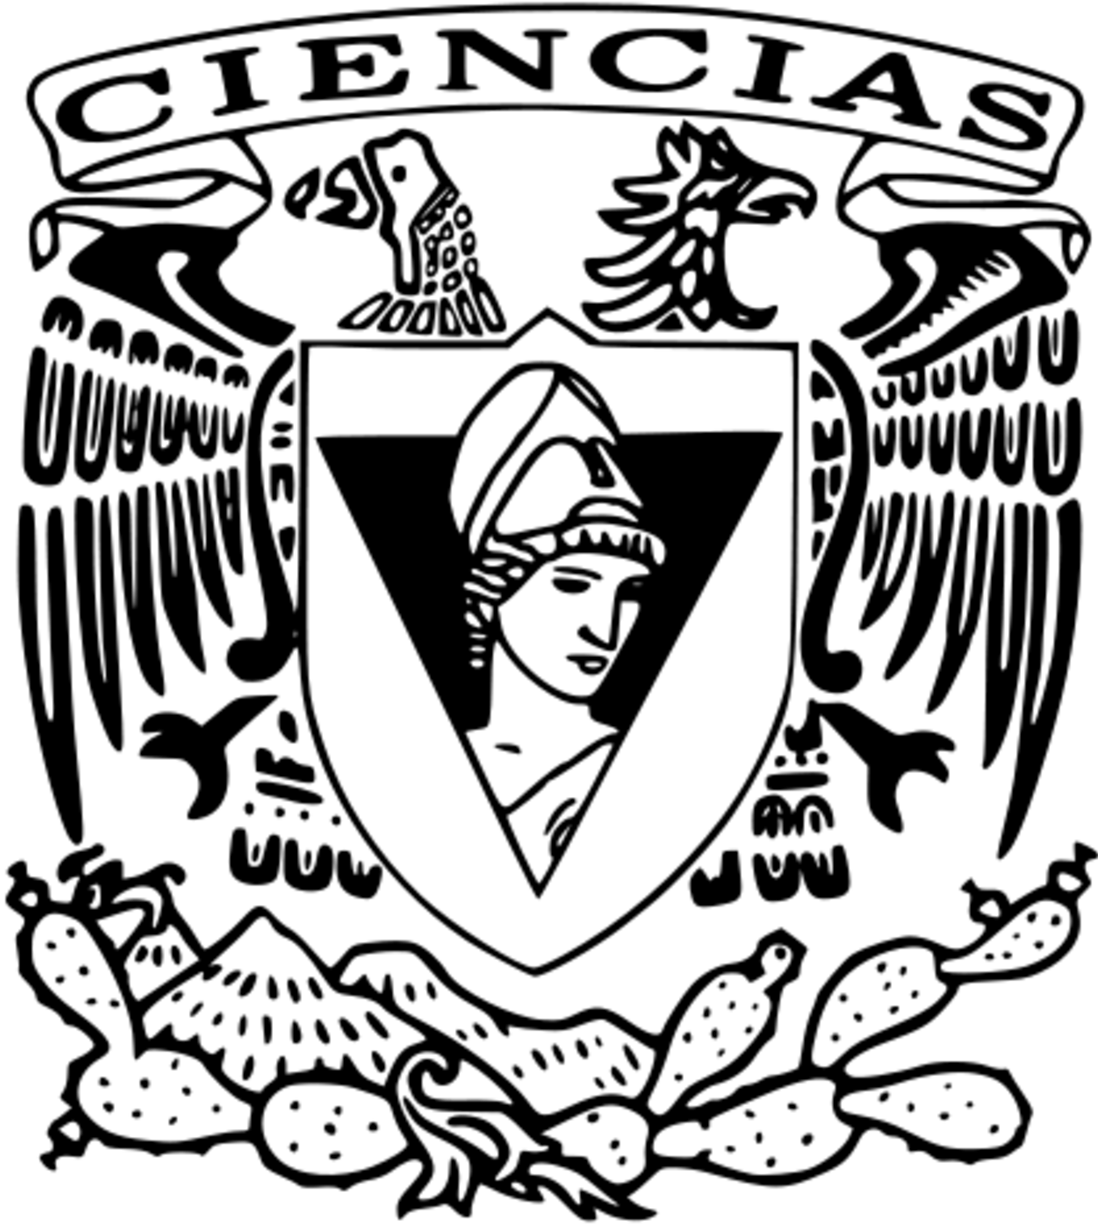
\includegraphics[height=4.0cm]{resources/Logo_FC.png}
		\end{center}
	\end{minipage}
	\begin{minipage}[c][0.81\textheight][t]{0.75\textwidth}
		\begin{center}
			\vspace{1cm}
			
			{\large\scshape Criptografía y Seguridad - 7133}\\[.2in]
			
			\vspace{2cm}            
			
			\textsc{\LARGE \textbf{P}\hspace{1cm}\textbf{R}\hspace{1cm}\textbf{A}\hspace{1cm}\textbf{C}\hspace{1cm}\textbf{T}\hspace{1cm}\textbf{I}\hspace{1cm}\textbf{C}\hspace{1cm}\textbf{A}\hspace{1.3cm}\textbf{1}}\\[2cm]
			\textsc{\Large{Equipo:}\normalsize \\
                \vspace{.3cm}
				\textbf{**** - 320083527 \\
                \vspace{.2cm}
				\href{https://github.com/JuanSosaCiencias}{{Sosa Romo Juan Mario - 320051926}} \\
                \vspace{.2cm}
				**** - 320017438 \\
                \vspace{.2cm}
                Sánchez Estrada Alejandro - 320335950 \\
                \vspace{.2cm}
                Ortega Medina David - 319111866}}\\[0.5cm]     
			
			\textsc{{Fecha de entrega: \\ \textbf{1 de Septiembre de 2025}}}\\[0.5cm]        
			
			\textsc{{Profesora: \\ \textbf{M. en C. Anayanzi Delia Martínez Hernández}}}\\[0.5cm]  
			
			\textsc{Ayudantes: \\ \textbf{Cecilia del Carmen Villatoro Ramos \\ José Angel Arévalo Avalos \\ David Armando Silva de Paz \\ Jesús Alberto Reyes Gutiérrez
			} }
			
			
			\vspace{0.5cm}
		\end{center}
	\end{minipage}
\end{titlepage}

    
    \begin{center}
	\section*{\LARGE{Practica 1}}
    \end{center}

    \begin{center}
        \LARGE{\textbf{Introducción}}\\
    \end{center}
    \normalsize
    La siguiente práctica tiene como objetivo aprender cómo funcionan los ataques y las vulnerabilidades relacionadas con SSH. Los puntos importantes de la práctica son los siguientes:

\begin{itemize}
  \item \textbf{Repaso de redes}
  \item \textbf{SSH}
  \item \textbf{Filtrado de diccionarios}
  \item \textbf{Daño colateral}
\end{itemize}

Además, durante la ejecución se hará uso intensivo de la terminal y de comandos UNIX para filtrar, depurar y atacar. Estos conceptos son de suma importancia, pues, además de formar parte de la práctica en términos de ataque, nos brindan buenas prácticas y pautas para mantener una defensa sólida y para desarrollar programas y sistemas más resistentes.


    
    \begin{center}
        \LARGE{\textbf{Desarrollo - Descifrado de archivos}}\\
    \end{center}
    \normalsize
    \begin{enumerate}
        \item \textbf{Descifrar el archivo file1.lol}
\begin{quote}
    Para el archivo \texttt{file1.lol} se comenzó inspeccionando su contenido binario en bruto,
    mostrando tanto los primeros caracteres en ASCII como en hexadecimal. El resultado
    no presentaba texto legible, sino bytes aparentemente aleatorios, lo que sugirió que se
    trataba de un cifrado clásico sobre bytes y no de una simple codificación.

    A continuación, se implementó un procedimiento en Python para probar de manera
    automática los cifrados César, Decimado y Afín, utilizando fuerza bruta sobre todas sus
    posibles claves. Una vez obtenido cada descifrado, se verificaba la cabecera con los
    \textit{magic bytes} característicos de distintos formatos (PDF, PNG, MP3, MP4).

    Para el caso del cifrado Afín, se utilizó la siguiente función que aplica la fórmula de
    descifrado con aritmética modular en $Z_{256}$:

    \vspace{.3cm}
    \begin{verbatim}
    def affine_decrypt(data, a, b):
        try:
            inv = pow(a, -1, 256)  # inverso modular de a
        except ValueError:
            return None
    
        result = bytearray()
        for byte in data:
            val = ((byte - b) * inv) % 256
            result.append(val)
        return result
    \end{verbatim}
    \vspace{.3cm}
    
    Tras las pruebas, se encontró que el método correcto era el \textbf{cifrado Afín} con
    parámetros $a=143$ y $b=157$. El archivo resultante comenzaba con la secuencia
    \texttt{0xFF 0xFB}, correspondiente al \textit{frame sync} de los archivos de audio MPEG
    Layer III (\texttt{.mp3}), lo que confirmó el formato.

    Una vez guardado el archivo descifrado, se verificó que podía reproducirse
    correctamente como audio. Con esto se validó el éxito del proceso de descifrado.
\end{quote}
\vspace{.5cm}

        \item \textbf{Ataque}

        \item \textbf{Descifrar el archivo file3.lol}

\begin{quote}
    Comencé por inspeccionar un poco el archivo utilizando un poco de código de Python:
    \vspace{.3cm}

    \begin{minted}[fontsize=\small, linenos, frame=single]{python}
def ascii_preview(b, length=512):
  s = b[:length]
  txt = ''.join(chr(x) if 32 <= x < 127 or x in (9,10,13) else '.' for x in s)
  return txt

print("=== ASCII preview")
print(ascii_preview(head, 512))
print("\n=== Hex ===")
print(' '.join(f"{x:02x}" for x in head[:128]))
    \end{minted}
    \vspace{.3cm}

    Como nota, todo el código que voy a mostrar para este procedimiento está incluido en el \texttt{p1CriptoEj3.ipynb} dentro del \texttt{src}.

    \begin{center}
    	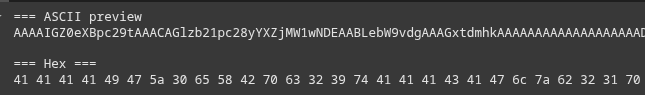
\includegraphics[width=.9\textwidth]{resources/ej3.png} 
    \end{center}

    De aquí, consulte con diversos LLMs para que me resaltaran el hecho de que todos los
    caracteres que encontré son imprimibles pertenecientes al alfabeto Base64 por lo que hice
    algunos tests para ver si se trataba de esta codificación. \vspace{.3cm}

    \begin{minted}[fontsize=\small, linenos, frame=single]{python}
# 1) bytes del head en base 64
only_b64 = all((c in B64_CHARS_WITH_NL) for c in head)
print("\n1) Bytes de head en b64?", only_b64)

# 2) padding con =
has_eq = b'=' in raw[-16:] or b'=\n' in raw or raw.rstrip().endswith(b'=')
print("2) Padding con =:", has_eq)

# 3) contar caracteres en ASCII
visible_chars = [c for c in head if 32 <= c < 127 or c in (9,10,13)]
if visible_chars:
    b64_count = sum(1 for c in visible_chars if c in B64_STD or c in (10,13))
    frac = b64_count / len(visible_chars)
else:
    frac = 0.0
print(f"3) Fraccion de contenido que es ASCII: {frac:.3f}")

# 4) Medir porcentaje de lineas longitud 4
lines = ascii_preview(raw, 4096).splitlines()
if lines:
    lengths = [len(l) for l in lines if len(l.strip())>0]
    if lengths:
        multiples_of_4 = sum(1 for L in lengths if L % 4 == 0)
        pct_mult4 = multiples_of_4 / len(lengths)
    else:
        pct_mult4 = 0.0
else:
    pct_mult4 = 0.0
print(f"4) Medir porcentaje de lineas longitud 4: {pct_mult4:.3f}")

# 5) Buscar firmas de formatos binarios
signs = []
if raw.startswith(b"%PDF"):
    signs.append("PDF")
if raw.startswith(b"\x89PNG\r\n\x1a\n"):
    signs.append("PNG")
if raw.startswith(b"\xff\xd8\xff"):
    signs.append("JPEG")
if raw.startswith(b"PK\x03\x04"):
    signs.append("ZIP")
print("5) Firmas de formatos binarios en el inicio:", signs if signs else "False")
    \end{minted}
    \vspace{.3cm}

    Dandome el siguiente resultado:
    \begin{center}
    	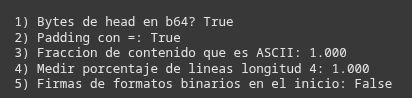
\includegraphics[width=.9\textwidth]{resources/ej3.2.png} 
    \end{center}

    Por estas métricas, todo indica que es base64. Como breviario cultural, la base 64 es una
    forma de codificar binario en texto de manera que los datos binarios están
    representados en secuencias de caracteres imprimibles usando el formato ASCII,
    específicamente cada 6 bits de los datos binarios de representan con un carácter del
    conjunto de 64 posibles. Es útil para transmitir datos binarios si solo podemos poner
    texto ademas, si la cadena no es del tamaño adecuado se utiliza el carácter de relleno $=$.
    Vemos que de las métricas recolectadas, todo parece apuntar a esta codificación.
    \vspace{.3cm}

    Hice un código que verifica con heurísticas si es base 64, e implemente una
    decodificación de base64, después busca en la cabeza del nuevo archivo los magic bytes para
    saber la extensión del archivo y después de saber que es \texttt{mp4} puse también
    código para poder verlo en el mismo notebook. Todo esto se puede ver en la ruta antes
    mencionada y aquí los resultados:

    \begin{center}
    	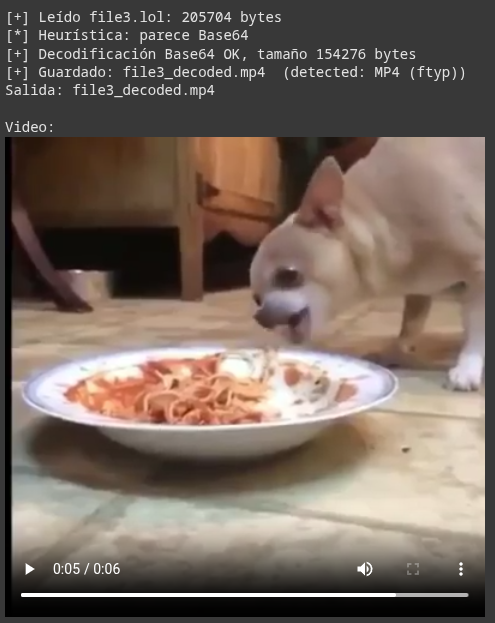
\includegraphics[height=12cm]{resources/ej3.3.png} 
    \end{center}

    Incluyo aquí también el decodificador: \vspace{.3cm}

    \begin{minted}[fontsize=\small, linenos, frame=single]{python}
def base64_decode_from_scratch(s):
  """
  Decodificador base64 desde cero.
  Acepta s como str (puede contener espacios/newlines).
  Devuelve bytes decodificados.
  """
  # Mantener solo chars válidos + '='
  s = ''.join(ch for ch in s if ch in _b64chars or ch == '=')
  if not s:
      return b''
  # Si la longitud no es múltiplo de 4, rellenar con '='
  pad_len = (4 - (len(s) % 4)) % 4
  if pad_len:
      s += '=' * pad_len

  out = bytearray()
  for i in range(0, len(s), 4):
      block = s[i:i+4]
      vals = []
      pad = 0
      for ch in block:
          if ch == '=':
              vals.append(0)
              pad += 1
          else:
              # Asumir 'A' (valor 0) si char inválido
              vals.append(_b64rev.get(ch, 0))
      # recomponer 24 bits
      triple = (vals[0] << 18) | (vals[1] << 12) | (vals[2] << 6) | (vals[3])
      b1 = (triple >> 16) & 0xFF
      b2 = (triple >> 8) & 0xFF
      b3 = triple & 0xFF
      out.append(b1)
      if pad < 2:
          out.append(b2)
      if pad == 0:
          out.append(b3)
  return bytes(out)
    \end{minted}
    \vspace{.3cm}
\end{quote} 
\vspace{.5cm}

        \item \textbf{Dentro de la red}

    \end{enumerate}
    

    \begin{center}
        \LARGE{\textbf{Desarrollo - preguntas}}\\
    \end{center}
    \normalsize
    \begin{enumerate}
        \item \textbf{¿Cuantos primos relativos hay en $\mathbb{Z}_{256}$?} \vspace{.3cm}

\begin{quote}
     Para responder esta pregunta voy a hacer uso de la
     función $\phi$ de Euler \citep{wikipedia_euler_totient_es}. La función $\phi (n) $ cuando
     $n=256=2^8$ cuenta la cantidad de enteros positivos menores o iguales a n que son
     primos relativos con este mismo:

     \begin{align*}
         \phi(p^k) &= p^k - p^{k-1} \\
         &= 2^8 - 2^7 \\
         &= 256 - 128 \\
         &= 128 \\
     \end{align*}

     Por tanto hay 128 enteros en el anillo que son primos relativos a $256$.
\end{quote}
\vspace{.5cm}

        \item \textbf{Sea $f: \mathbb{Z}_n \rightarrow \mathbb{Z}_n$ tal que $f(i)=k * i$ para $i \in A$ con $A$ un alfabeto cualquiera ?`qu\'e se debe de cumplir para que $f$ sea una funci\'on biyectiva?}\\\\
Tenemos la función  
\[
f:\mathbb{Z}_n \to \mathbb{Z}_n, \quad f(i)=k \cdot i \pmod n
\]
donde \(\mathbb{Z}_n\) son los enteros módulo \(n\) (los números \(0,1,2,\dots,n-1\)), y \(k\) es un número fijo.  
\\\\
Para que \(f\) sea biyectiva debemos de cumplir dos cosas:\\  
1. Inyectiva: que no haya dos elementos distintos que se manden al mismo resultado.\\  
2. Sobreyectiva: que todos los elementos de \(\mathbb{Z}_n\) se puedan obtener como imagen de alguno.  
\\\\
Es un conjunto finito, sol debemos de revisar la inyectividad: si la función no repite valores, entonces será sobreyectiva.  
\\\\\\  
Si tomamos dos elementos \(i\) y \(j\) y resulta que \(f(i) = f(j)\), entonces
\[
k \cdot i \equiv k \cdot j \pmod{n}.
\]
Esto se simplifica a  
\[
k \cdot (i-j) \equiv 0 \pmod{n}.
\]
Lo que significa que \(n\) divide a \(k \cdot (i-j)\).  
\\\\
Aquí aparece el máximo común divisor \(\gcd(k,n)\):\\  
- Si \(\gcd(k,n) = d > 1\), entonces es posible que \(i \neq j\) pero aún así \(k(i-j)\) sea múltiplo de \(n\). En este caso la función no es inyectiva.  \\
- Si \(\gcd(k,n)=1\), no hay divisores comunes, y la única forma de que \(k(i-j)\) sea múltiplo de \(n\) es que \(i-j\) lo sea. Es decir, si \(i\neq j\), sus imágenes no se confunden.  \\
En conclusión, la función $f(i) = k \cdot i \pmod{n}$ es biyectiva si y sólo si
\[
\gcd(k,n) = 1.
\]
\citep{lec_7_handout}

        \item \textbf{¿Cuántas posibles combinaciones no triviales existen para cifrar bytes con César, Decimado y Afin?}\\\\
Primero nos surge la duda de que nos referimos con "no triviales", con eso en mente, vamos a intentar responder lo mejor posible. \\
\textbf{Cifrado C\'esar}:
\begin{enumerate}
    \item Combinaciones no triviales: 255
    \item Nuestro razonamiento es el siguiente, con 256 valores posibles (0-255) habr\'a 256 desplazamientos totales, excluimos el dezplazmaiento 0, trivial, nos quedan 255 \'utiles, en el alfabeto de 26 letras siguiendo la misma regla hay 25 desplazamientos utiles, , entonces para 256 simbolos, los que consideramos no triviales son 256-1=255 \citep{dCOde}
\end{enumerate}
\textbf{CifradoDecimado}
\begin{enumerate}
    \item COmbinaciones no triviales: 127
    \item NUestro razonamiento, este cifrado usa la fórmula $C = aM \bmod 256$, donde $a$ debe ser coprimo con $256$. El número de enteros coprimos con $256$ es $\varphi(256)=128$. Excluyendo la clave trivial $a=1$ (identidad), quedan $128 - 1 = 127$ combinaciones no triviales. \citep{wikipedia_euler_totient_es}
\end{enumerate}
\textbf{Cifrado Af\'in}
\begin{enumerate}
    \item COmbinaciones no triviales: 32767
    \item El cifrado afín usa la fórmula $C = aM + b \bmod 256$. Con $n=256$ hay $\varphi(256)=128$ valores posibles de $a$ (coprimos con $256$) y $256$ valores posibles para $b$, resultando en $128 \times 256 = 32768$ pares clave totales. Al excluir la clave identidad $(a=1, b=0)$, quedan $32768 - 1 = 32767$ combinaciones no triviales.\citep{Course_SideKick}
\end{enumerate}

        \item \textbf{}
        \item \textbf{¿Por qué los archivos descifrados tienen exactamente el mismo tamaño antes de cifrar
pero no pudimos leerlos? ¿Por qué no tuvimos que agregar/quitar nada?}

\begin{quote}
    Lo primero que hay que recordar es que estamos usando cifrados en donde reemplazamos o
    reacomodamos la información original, por ejemplo con sustituciones 1 a 1 entre letras o en
    el caso de base64 solo codificamos (aunque esto si aumenta el tamaño) porque usamos 4
    caracteres por cada 3 bytes pero regresa al mismo tamaño al descifrar. \vspace{.3cm}

    El que no se pueda leer es porque los programas que se utilizan para leer estos archivos
    esperan cierto formato en los archivos, especialmente cuando ven la firma y buscan los magic
    bytes para saber como leerlo, entonces al modificar las estructuras y los bytes que
    utilizan para decodificarlo la información queda de cierta manera inutilizada.
    \vspace{.3cm}

    En cuanto a agregar a eliminar cosas vamos por casos:
    \begin{enumerate}
        \item César, Decimado, Afín: esto es sustitución monoalfabetica 1 a 1 por lo que el
            tamaño no debe cambiar y no es necesario quitar o añadir nada.
        \item B64: Esto como ya dijimos es una reacomodación de la información en bloques,
            si se agrega el carácter de padding usualmente \texttt{=} pero al decodificar
            se omite este mismo por lo que no se quita ni agrega nada.
    \end{enumerate}

    De manera concisa podríamos decir que las operaciones que usamos son biyectivas sobre el
    conjunto de símbolos. 
\end{quote}
\vspace{.5cm}

        \item \textbf{Ya que \textit{base64} no es un cifrado, sino codificación, ¿en qué casos podemos usarlo?}\\

Base64 nos sirve para representar datos binarios en texto ASCII, y esto es útil cuando un canal de comunicación unicamente permite caracteres imprimibles, los casos en los que sería útil usar Base64 son:
\begin{itemize}
    \item{Para transmitir datos binarios en canales de texto, por ejemplo enviar imágenes en correos electrónicos.}
    \item{Para incluir datos binarios en un JSON o XML, por ejemplo incrustar una imagen un una respuesta JSON para un API.}
    \item{Para Codificar datos para URLs, por ejemplo, evitar caracteres inválidos o reservados un una URL}
\end{itemize}
    \end{enumerate}

    \begin{center}
        \LARGE{\textbf{Conclusiones}}\\
    \end{center}
    \normalsize
    


    
\newpage

\Large \section*{Bibliografía}
  \bibliography{resources/referencias/referencias}
  \bibliographystyle{plainnat}
  
    
	

\end{document}
